\documentclass[aspectratio=1610, 13pt]{beamer}
\usepackage{xcolor}
\usepackage{multicol}
\usepackage{mathtools,array}
\usepackage[T1]{fontenc}

\usepackage{stmaryrd}
\usepackage{dutchcal}
\usepackage{zi4}
\usepackage[font={scriptsize,bf}]{caption}
% \usepackage{subcaption}
\usepackage{graphics}
\usepackage{tikz}
\usepackage{fontawesome5}
\usepackage{mathpartir}

\newcommand{\naturals}{\mathbb{N}}
\newcommand{\reals}{\mathbb{R}}

\newcommand{\Dist}[1]{\mathcal{D}(#1)}
\newcommand{\expectation}{\mathbb{E}}

\newcommand{\states}{S}
\newcommand{\actions}{A}
\newcommand{\observables}{O}
\newcommand{\trans}{T}
\newcommand{\obs}{Z}
\newcommand{\reward}{R}
\newcommand{\discount}{\gamma}

\newcommand{\beliefs}{\mathcal{B}}
\newcommand{\beliefUpdate}{\tau}

\newcommand{\policy}{\pi}

\newcommand{\diff}[1]{\mathop{}\!\mathrm{d}#1}
\renewcommand{\figurename}{Figure}
\renewcommand{\refname}{Reference}

\AtBeginDocument{
  \catcode`_=12
  \begingroup\lccode`~=`_
  \lowercase{\endgroup\let~}\sb
  \mathcode`_="8000
}

% \usetheme{Madrid}
% % \usetheme{default}
% \setbeamertemplate{caption}[numbered]
% \setbeamerfont{title}{size=\large}
\mode<presentation>
{
  \usetheme{Darmstadt}      % or try Darmstadt, Madrid, Warsaw, ...
  \usecolortheme{default} % or try albatross, beaver, crane, ...
  \usefonttheme[onlymath]{serif}  % or try serif, structurebold, ...
  \setbeamertemplate{navigation symbols}{}
  \setbeamertemplate{caption}[numbered]
  \setbeamertemplate{footline}[frame number] 
} 

\usepackage{listings}
\lstdefinestyle{heaplang}{
    language=Caml,
    basicstyle=\footnotesize\ttfamily,
    keywordstyle=\color{blue},
    commentstyle=\color{red},
    escapeinside={<@}{@>},
    morekeywords={new_chan, fork, recv, send, swap, ref}
}
\lstdefinestyle{clang}{
    language=Caml,
    basicstyle=\footnotesize\ttfamily,
    keywordstyle=\color{blue},
    commentstyle=\color{red},
    escapeinside={<@}{@>},
}
\lstset{style=heaplang}

\usepackage{natbib}

\newcommand{\buchi}{B\"uchi }

\definecolor{goldenpoppy}{rgb}{0.99, 0.76, 0.0}
\definecolor{goldenyellow}{rgb}{1.0, 0.87, 0.0}
\definecolor{green2}{rgb}{0.1,0.7,0.3} 
\newcommand{\gcheck}{{\color{green2}\faCheckCircle[regular] }}
\newcommand{\rcross}{{\color{red} \faTimesCircle[regular]} }
\newcommand{\rflag}{{\color{red} \faFlag}}
% \usepackage{algorithm,amsmath}
% \usepackage[noend]{algpseudocode}

\newcommand{\zlstinline}{\let\par\endgraf\lstinline}
\newcommand{\comments}[1]{{\color{red}#1}}
\title{SAT-Based Model Checking Without Unrolling}
\author{Author: Aaron R. Bradley\\
Reporter:  Xie Li}
\date{\today}
\begin{document}
\maketitle
\begin{frame}{IC3/PDR: Related Papers}
\begin{itemize}
\item Checking Safety by Inductive Generalization of
Counterexamples to Induction
\item SAT-Based Model Checking Without Unrolling
\item Understand IC3
\item Efficient implementation of property directed reachability
\end{itemize}
\end{frame}

\begin{frame}{Overview}
\begin{itemize}
\item Preliminaries
\item Introduction to a Naive Model Checker FSIS:
	\begin{itemize}
	\item The Idea
	\item Algorithm: \texttt{LIC} and \texttt{MIC}
	\item Observations.
	\end{itemize}
\item Introduction to IC3:
\begin{itemize}
\item The Idea.
\item Description of the algorithm.
\end{itemize}
\end{itemize}
\end{frame}

\begin{frame}{Preliminaries: Propositional Logic}
	\begin{itemize}
	\item \textbf{Literal}: A literal $l$ is a propositional variable or its negation: $x, \neg y$.
	\item \textbf{Clause}: A clause $c$ is a disjunction of literals. We use $|c|$ to denote the size of a clause, i.e. the number of literals in the clause.
	\item \textbf{Subclause}: A subclause $d$ of a clause $c$ is a disjunction of a subset of literals of $c$. abbr. $d \sqsubseteq c$
	
	$c: x\vee y \vee \neg z, d: x\vee \neg z$. 
	\end{itemize}
\end{frame}
\begin{frame}{Preliminaries: Transition System}
\begin{definition}[Boolean Transition System]
A boolean transition system $\mathcal{S} = \langle \bar{x}, \theta, \rho\rangle$ has three component where:

\begin{itemize}

\item $\bar{x} = \{x_1, x_2, \ldots, x_n\}$ is the set of propositional variables that are assigned true.
\item $\theta(\bar{x})$ is a propositional formula stating the initial condition.
\item $\rho(\bar{x}, \bar{x}')$ is a propositional formula describing the transition relation.

\end{itemize}
\end{definition}
The semantic of a transition system is given by its computations:
\begin{definition}[State and Computation]
\begin{itemize}
\item A \textit{state} $s$ of a boolean transition system $\textsc{S}$ is an assignment of the variables $\bar{x}$.
\item A computation $\sigma: s_0, s_1, s_2, \ldots
$ is a sequence of states satisfying initial condition and transition relations: 

$\theta(s_0) \wedge \forall i \ge 0. \rho(s_i, s_{i+1}) \equiv T$.
\end{itemize}

\end{definition}
\end{frame}

\begin{frame}{Preliminaries: Subclause Lattice}
Consider an clause $c$ and its induced subclause lattice $L_c = \langle 2^c, \sqcap, \sqcup, \sqsubseteq \rangle$ where 
\begin{itemize}
\item Elements of $2^c$ are subclauses of $c$,
\item Elements are ordered by the subclause relation $\sqsubseteq$ ,
\item Join operator $\sqcup$ is just disjunction, and
\item Meet operation $\sqcap$ is the disjunction of common literals.
\end{itemize}

By Tarski theorem,  every monotone function on $L_c$ has a least fixpoint and 	greatest fixpoint.


\end{frame}

\begin{frame}{Preliminaries: Inductive Invariant}
\begin{definition}[Inductive Invariant]
A formula $\varphi$ is an inductive invariant on $\mathcal{S}$ if
\begin{itemize}
\item it holds initally: $\theta \Rightarrow \varphi$
\item and it is preserved under transition: $\varphi \wedge \rho \Rightarrow \varphi'$

\end{itemize}
\end{definition}

A formula $\varphi$ is \textbf{inductive related to }an inductive formula $\psi$ if
\begin{itemize}
\item it holds initally: $\theta \Rightarrow \varphi$
\item and $\psi \wedge \varphi \wedge \rho \Rightarrow \varphi'$
\end{itemize}
\end{frame}



\begin{frame}{Introduction to FSIS}
\begin{center}

FSIS: Finite-State Inductive Strengthening
\end{center}

\textbf{Problem}: 

Given a transition system $\mathcal{S}$ and specification formula $\Pi$, is $\Pi$ an invariant on $\mathcal{S}$?


FAQ:
\begin{itemize}
\item Why does this problem matter?
\item Where does ``strengthening'' comes from?

$\Pi$ usually is an invariant not inductive, we wish to find a \textit{strengthening assertion} $\chi$ such that $\Pi\wedge \chi$ is inductive.
\end{itemize}


Basic Idea: generating many clauses, each of which is inductive related to previous-generated clause. Later use them to construct $\Pi\wedge \chi$
\end{frame}

\begin{frame}{Introduction to FSIS}

\end{frame}


\begin{frame}{Introduction to FSIS}

\end{frame}


\begin{frame}{Introduction to FSIS}

\end{frame}

\begin{frame}{Introduction to FSIS}

\end{frame}

\begin{frame}{LIC and MIC: Compute Minimal Inductive Subclause}
\texttt{down}$(L_c, d)$:

Given a subclause lattice $L_c$ and the clause $d$, return the unique largest subclause $e\sqsubseteq d$ such that the implication $\psi \wedge e \wedge \rho \Rightarrow d'$ holds: use counterexample to shrink the space.


\texttt{LIC}$(L_c, c)$: applies \texttt{down} several times.
\begin{itemize}
\item If the implication $\psi \wedge c \wedge \rho \Rightarrow c'$ and $\theta \Rightarrow c$ holds, the return $c$.
\item If it does not hold, $\psi\wedge c \wedge \rho \wedge \neg c'$ is satisfied by some assignment $(s, s')$.

\item Let $\neg t$ be the best over-approximation of $\neg s$ in $L_c$ and compute a new clause $d = c \sqcap \neg t$.

\item Recurse on $d$.
\end{itemize}

\end{frame}

\begin{frame}{LIC and MIC: Compute Minimal Inductive Subclause}
\begin{theorem}[Large Inductive Subclause]
The fixpoint of the iteration sequence computed by \texttt{LIC}$(L_c, c)$ is the largest subclause of $c$ that satisfies consecution. If it also satisfies initiation, then it is the largest inductive subclause of $c$. Finding it require at most $O(|c|)$ SAT queries.

\end{theorem}

Let the computed sequence be $c_0 = c, c_1, \ldots , c_k$.

Suppose $e \sqsubseteq c$ also satisfies consecution but is not a subclause of $c_k$:

Let $i$ be the position that 
\[e \sqsubseteq c_i \wedge e \not \sqsubseteq c_{i + 1}\]

Partition $c_i$ into $e\vee f$ where $f$ contains only literals from $c_i$.

The consecution is not satisfied: $\psi \wedge (e\vee f) \wedge \rho \wedge \neg (e' \vee f')$ is satisfied by $(s, s')$
\begin{itemize}
\item $\psi \wedge e \wedge \rho \wedge \neg e' \wedge \neg f'$
\item $\psi \wedge \neg e \wedge f \wedge \rho \wedge \neg e' \wedge f'$
\end{itemize}

$\neg e$ is true under the assignment $s$, hence $e \sqsubseteq \neg s$. Contradiction.
\end{frame}

\begin{frame}{LIC and MIC: Compute Minimal Inductive Subclause}

\texttt{MIC}$(\mathcal{S}, \psi, c)$: returns a minimal subclause of $c$ that is inductive related to $\psi$.

\begin{center}
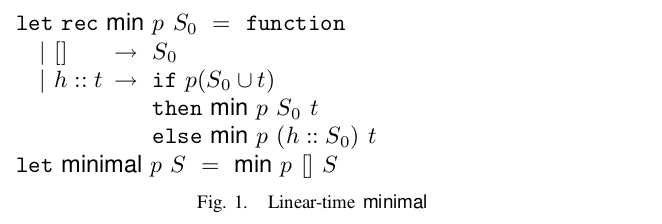
\includegraphics[scale=0.4]{pic1.png}
\end{center}

\begin{theorem}[Correct]
The algorithm terminates and returns the minimal $\bar{S}$ s.t. $p(\bar{S})$ is true.
\end{theorem}
\end{frame}

\begin{frame}{Obsevation of FSIS}
\begin{itemize}
\item The algorithm can be implemented to find inductive clauses in parallel.
\item The algorithm enters long searches for the next relatively inductive clause
\item An unreachable state may not have a inductive generalization.
\item Not making good use of stepwise information.
\end{itemize}
\end{frame}

\begin{frame}\frametitle{Introduction to IC3}
\begin{center}

\textbf{IC3:} Incremental Construction of Inductive Clauses for Indubitable Correctness.
\end{center}


Data structure: A sequence of formulas

\[F_0, F_1, F_2, \ldots, F_k\]


\begin{itemize}
\item $\theta \Rightarrow F_0$
\item $F_i\Rightarrow F_{i + 1}$
for $0\le i < k$
\item $F_i\Rightarrow \Pi$
for $0\le i \le k$
\item $F_i\wedge \rho \Rightarrow F_{i + 1} '$ 
for $0\le i < k$
\end{itemize}

We use $\text{clause}(F_i)$ to denote the set of clauses that comprises $F_i$: $F_i = \Pi \wedge \bigwedge \text{clause}(F_i)$.

\end{frame}


\begin{frame}{Introduction to IC3}

\end{frame}
\begin{frame}{Introduction to IC3}

\end{frame}
\begin{frame}{Introduction to IC3}

\end{frame}
\begin{frame}{Introduction to IC3}

\end{frame}


\begin{frame}{Description of the Algorithm}



\begin{itemize}
\item First check whether $\theta \wedge \neg \Pi$ or $\theta \wedge \rho \wedge \Pi'$ is satisfiable to detect counterexample.

\item Major iteration: 

\begin{itemize}

\item If $F_k \wedge \rho \Rightarrow \Pi'$, then enter major iteration $k + 1$ and let $F_{k + 1} = \Pi$.

\item For any clause $c\in F_i$, $0 \le i \le k$, if $F_i \wedge \rho \Rightarrow c'$ and $c \not\in \text{clauses}(F_{i+1})$, then $c$ is conjoined to $F_{i + 1}$.

\item If ever $F_i = F_{i + 1}$, the proof is complete and  $\Pi$ is an invariant.
\end{itemize}
\item Minor iteration: Suppose $F_k\wedge \rho \not\Rightarrow \Pi'$:

\begin{itemize}
\item Let the counterexample be $s$ and find the greatest $F_i$ s.t. $\neg s$ is inductive related to $F_{i}$. Then a strengthening $c \sqsubseteq \neg s$ will be conjoined to $F_0, \ldots, F_{i + 1}$. 

\item If $i = k$ or $i = k - 1$, then after conjoining $F_k \wedge \rho \Rightarrow \Pi'$.
\item Otherwise there is a state $t\in F_{i + 1}$ but $t\not\in F_{i}$.




\end{itemize}
\end{itemize}
\end{frame}

\end{document}